% Q14 -- 4-bit ALU: adder cascade with the carry-in line used as the function (mode) select.
\documentclass[border=10pt]{standalone}
\usepackage{tikz}
\usetikzlibrary{arrows.meta}
\begin{document}
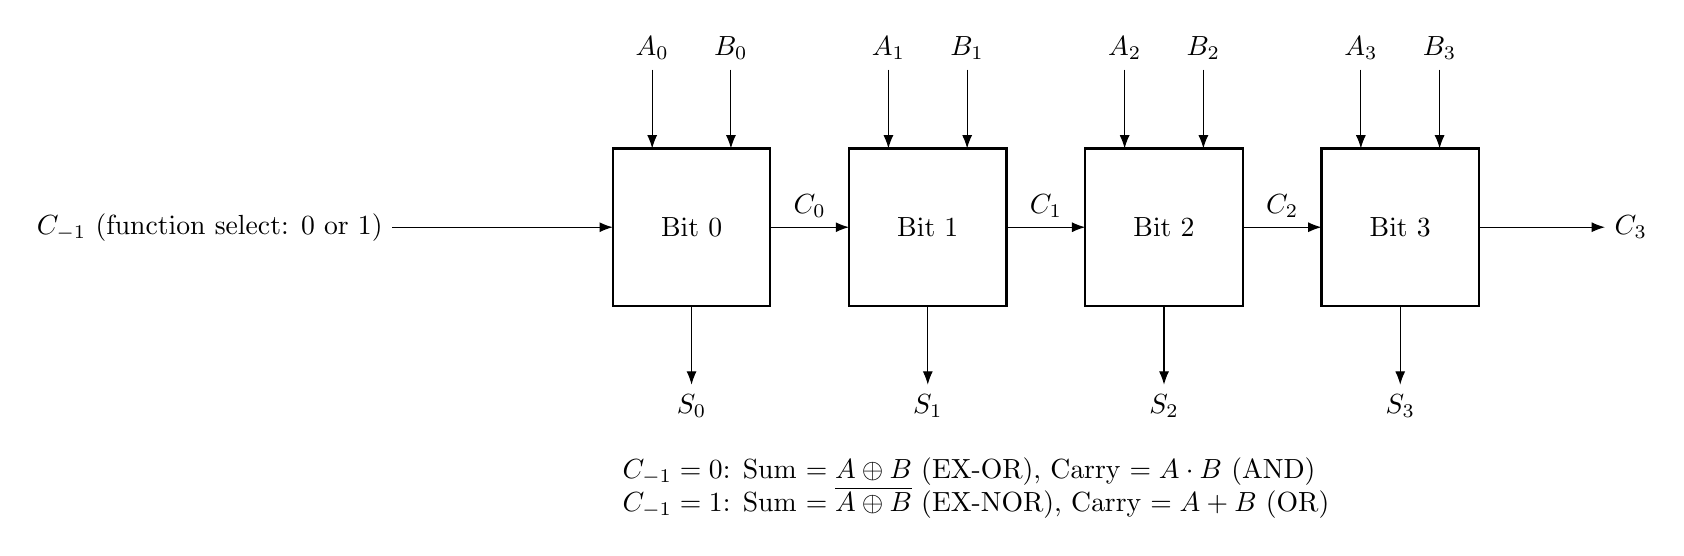
\begin{tikzpicture}[>=Latex]
\draw[thick] (0,0) rectangle (2,2);  \node at (1,1) {Bit 0};
\draw[->] (0.5,3) node[above]{$A_0$} -- (0.5,2);
\draw[->] (1.5,3) node[above]{$B_0$} -- (1.5,2);
\draw[->] (1,0) -- (1,-1) node[below]{$S_0$};
\draw[thick] (3,0) rectangle (5,2);  \node at (4,1) {Bit 1};
\draw[->] (3.5,3) node[above]{$A_1$} -- (3.5,2);
\draw[->] (4.5,3) node[above]{$B_1$} -- (4.5,2);
\draw[->] (4,0) -- (4,-1) node[below]{$S_1$};
\draw[thick] (6,0) rectangle (8,2);  \node at (7,1) {Bit 2};
\draw[->] (6.5,3) node[above]{$A_2$} -- (6.5,2);
\draw[->] (7.5,3) node[above]{$B_2$} -- (7.5,2);
\draw[->] (7,0) -- (7,-1) node[below]{$S_2$};
\draw[thick] (9,0) rectangle (11,2); \node at (10,1) {Bit 3};
\draw[->] (9.5,3) node[above]{$A_3$} -- (9.5,2);
\draw[->] (10.5,3) node[above]{$B_3$} -- (10.5,2);
\draw[->] (10,0) -- (10,-1) node[below]{$S_3$};
\draw[->] (-2.8,1) node[left]{$C_{-1}$ (function select: 0 or 1)} -- (0,1);
\draw[->] (2,1) -- (3,1);  \node[above] at (2.5,1){$C_0$};
\draw[->] (5,1) -- (6,1);  \node[above] at (5.5,1){$C_1$};
\draw[->] (8,1) -- (9,1);  \node[above] at (8.5,1){$C_2$};
\draw[->] (11,1) -- (12.6,1) node[right]{$C_3$};
\node[align=left, anchor=north west] at (0,-1.8)
  {$C_{-1}=0$: Sum $=A\oplus B$ (EX-OR), Carry $=A\cdot B$ (AND)\\
   $C_{-1}=1$: Sum $=\overline{A\oplus B}$ (EX-NOR), Carry $=A+B$ (OR)};
\end{tikzpicture}
\end{document}
